%tex
%% $Id: anleitung.tex 74 2009-07-30 18:39:03Z miracle $
\documentclass[ngerman,12pt]{tumbook}
\usepackage{subfigure}
\usepackage{float}

%\raster

\makeindex
\newcommand{\bs}{\textbackslash}
\newcommand{\fn}[1]{,,\textsl{#1}``}
\newcommand{\cmd}[1]{\textbf{#1}}
\newcommand{\slcmd}[1]{\cmd{\textbackslash#1}}

\newcommand{\MiKTeX}{MiK\TeX{}}
\newcommand{\TeXLive}{\TeX{}Live}
\newcommand{\email}[1]{\textbf{\textsl{#1}}}
\newcommand{\maintainers}{\email{tum@as-computer.de}}
\newcommand{\ediseppmail}{\email{tum@ediundsepp.de}}
\newcommand{\tumcdurl}{http://www.tumcd.de/}
\newcommand{\subnav}{\guillemotright}

\Semester{WS 2009/2010}
\title{Arbeiten mit den TU-\LaTeX{}-Vorlagen}
\Untertitel{Eine kurze Anleitung zum Umgang mit tumbook.cls\\zur Erstellung von wissenschaftlichen Arbeiten f\"ur die TU M\"unchen}
\Themensteller{\textsl{ediundsepp} GbR Gestaltungsgesellschaft, M�nchen}
\TUMAdresse{}
\Autorenadresse{AS Computer Consulting \& Service GmbH, M\"unchen}
\Abgabetermin{31. Juli 2009}
\author{Ulrike Schrepf und Jan Schormann}
\date{M\"unchen, den \today}
\begin{document}
\maketitle
\tableofcontents

\clearpage

\chapter{Einleitung}

Dies ist ein Paket von Schriftartdateien und \LaTeX{}-Klassen,
die zusammen das Erstellen von Briefen und Faxnachrichten im Corporate Design
der Technischen Universit"at M"unchen erlauben.

\vspace{\baselineskip}

Das Corporate Design ist hier beschrieben: \tumcdurl{} \\
Bei Fragen zur Gestaltung: \ediseppmail{} \\
Bei Fragen zu den \LaTeX{}-Dokumenten oder zur Installation: \maintainers{}

Die Anleitung zur Installation finden Sie in Abschnitt~\ref{install} am Schluss dieses Dokuments.

\chapter{Grundlagen}

Bei \fn{tumbook.cls} handelt es sich um eine Abwandlung der bekannten
Dokumentklasse \fn{book.cls}. Die grundlegenden Bestandteile dieser Klasse blieben
dabei erhalten. Einige Optionen wurden allerdings durch fixe Vorgaben ersetzt
und weitere f"ur wissenschaftliche Arbeiten bei der TU typische Angaben wurden
in den Variablensatz "ubernommen.

Beim Arbeiten mit \fn{tumbook.cls} kann man also weitgehend die
Features der book-Dokumentklasse nutzen.

Einige Features der Bookklasse wurden mit Absicht ausgestellt. Dabei handelt
es sich um:
\begin{enumerate}
\item die Papierwahl -- nun voreingestellt auf DIN~A4.
\item die Titelseite -- nun immer auf einem eigenen Blatt.
\item die Kopfzeilen -- nun immer mit Seitenzahl in der Mitte.
\end{enumerate}

\section{Integrierte Pakete}

Folgende Pakete wurden in f"ur die Dokumentklasse bereits importiert, und lassen
sich damit ohne expliziten Eigenimport direkt nutzen:

\cmd{babel}\quad
\cmd{calc}\quad
\cmd{color}\quad
\cmd{epsfig}\quad
\cmd{float}\quad
\cmd{inputenc}

\chapter{Dokumenterstellung}

F"ur die Erstellung von Dokumenten f"ur die TU M"unchen werden einige spezielle
Anpassungen ben"otigt. Weitgehend wurde aber versucht auf die Standardkommandos
von \LaTeX{} zur"uckzugreifen, um erfahrenen \LaTeX{}-Benutzern die Arbeit
zu erleichtern und Einarbeitungszeiten zu verk"urzen.

\section{Vorarbeiten}

Einige der relevanten Informationen zu Dokument und Verarbeitung werden "uber
Optionen gesetzt oder in der Pr"aambel vereinbart. In diesem Abschnitt finden
Sie eine Liste dieser Optionen und Daten.

\subsection{Optionen}

Folgende Optionen sollten bei der Dokumentklasse gesetzt werden. Abh"angig von den
eingesetzten Paketen sind weitere Optionen m"oglich.

\begin{table}[H]
\center{
\begin{tabular}{|l|p{.32\textwidth}|p{.28\textwidth}|p{.13\textwidth}|}
\hline
\multicolumn{4}{|c|}{Optionsliste}\\ \hline
\textbf{Name/Art} & \textbf{Beschreibung}  & \textbf{m"ogliche Werte} & \textbf{Standard} \\  \hline
Encoding & \raggedright Im Text verwendete Zeichen; passend zu dieser Angabe werden Sonderzeichen interpretiert.
& \cmd{latin1, latin2, utf8,} \dots & --- \\ \hline
Sprache & \raggedright Spracheinstellung f"ur das Babel-Paket. & \raggedright \cmd{ngerman, english,} \dots & ---\\ \hline
Fakult"at & \raggedright Fakult"at f"ur die die Arbeit erstellt wurde;  bestimmt das Logo &
\raggedright \cmd{NEUTRAL, AR, BV, CH, EI, IN, MW, MA, MED, PH, SE, SP, WI, WZW} & \cmd{NEUTRAL} (kein Logo)\\ \hline
Schriftgr"o"se & \raggedright In der Arbeit verwendete Schriftgr"o"se & \cmd{9pt, 10pt, 12pt} & \cmd{10pt} \\ \hline
\end{tabular}}
\caption{Optionen f"ur die Dokumentklasse}
\end{table}

\subsection{Die Pr"aambel}

Folgende Daten sollten in der Pr"aambel gesetzt werden:

\begin{table}[H]
\center{
\begin{tabular}{|l|p{.55\textwidth}|c|}
\hline
\multicolumn{3}{|c|}{Pr"aambeldaten}\\ \hline
\textbf{Name} & \textbf{Beschreibung} & \textbf{obligatorisch} \\ \hline
\cmd{Seminar} & Seminartitel zur Arbeit & --- \\ \hline
\cmd{Semester} & Semester f"ur das die Arbeit geschrieben wurde & --- \\ \hline
\cmd{title} & Titel der Arbeit & x \\ \hline
\cmd{Untertitel} & Untertitel zur Arbeit & ---\\ \hline
\cmd{Themensteller} & Verantwortlicher Dozent & --- \\ \hline
\cmd{Autorenadresse} & Anschrift des Autors der Arbeit & --- \\ \hline
\cmd{Abgabetermin} & Verpflichtender Termin zur Abgabe & ---\\ \hline
\cmd{author} & Autor der Arbeit& x\\ \hline
\cmd{date} & Ort und Datum der Erstellung,
wird auch f"ur ehrenw"ortliche Erkl"arung eingesetzt & x \\ \hline
\cmd{Matrikelnummer} & Matrikelnummer des Autors
(ggf. mittels \LaTeX\-Befehlen gegliedert z.B. \slcmd{,}) & ---\\ \hline
\cmd{Fachsemester} & Fachsemester des Autors passend zum
angegebenen Semester oben & --- \\ \hline
\end{tabular}}
\caption{Informationen in der Pr"aambel}
\end{table}

\section{Aufbau des Dokuments}
Hier folgt eine Liste der Anpassungen, die zur Erstellung eines \textit{tumbooks} notwendig
sind. Die Bereiche des Dokuments entsprechen weitesgehend der Dokumentklasse \fn{book.cls}.

\subsection{Titelblatt}

Das Titelblatt wird wie gewohnt mit \slcmd{maketitle} erzeugt.
Das Titelblatt bekommt immer eine eigene Seite. Anders als bei \fn{book.cls}
gibt es bei \fn{tumbook.cls} keine Option \cmd{titlepage}.

Auf der Titelseite wird das Logo der TU und das Logo der Fakult"at angezeigt, wenn diese
"uber die Optionen korrekt ausgew"ahlt wurde.

\begin{figure}[H]
\center{
\subfigure{
\label{archlogo}
    
\epsfig{file=AR.pdf,height=9.605mm}
}
\subfigure{
    
\epsfig{file=BV.pdf,height=9.605mm}
}
\subfigure{
    
\epsfig{file=CH.pdf,height=9.605mm}
}
\subfigure{
    
\epsfig{file=EI.pdf,height=9.605mm}
}
\subfigure{
    
\epsfig{file=IN.pdf,height=9.605mm}
}
\subfigure{
   
\epsfig{file=MW.pdf,height=10.1mm,viewport=2.3mm 0mm 13.6mm 11mm}
}
\subfigure{
    
\epsfig{file=MA.pdf,height=9.605mm}
}
\subfigure{
    
\epsfig{file=MED.pdf,width=9.605mm,viewport=0mm 2.7mm 10.5mm 13.4mm}
}
\subfigure{
    
\epsfig{file=PH.pdf,height=9.605mm}
}
\subfigure{
    
\epsfig{file=SE.pdf,height=9.605mm}
}
\subfigure{
    
\epsfig{file=SP.pdf,height=10.065mm,viewport=2mm 0mm 13.4mm 11mm}
}
\subfigure{
    
\epsfig{file=WI.pdf,height=9.605mm,viewport=0.65mm 0mm 10.9mm 10.5mm}
}
\subfigure{
    
\epsfig{file=WZW.pdf,height=9.605mm}
}
\caption{Logos der TU M"unchen}\label{logos}}
\end{figure}


\subsection{"Uberschriften}

Innerhalb des Dokuments werden die "Uberschriftsebenen "uber \slcmd{chapter},
\slcmd{section}, \slcmd{subsection}, \slcmd{subsubsection} strukturiert.
Alle vier "Uberschriftsebenen werden im Inhaltsverzeichnis sichtbar.

Die Schriftgr"o"sen sind dabei entsprechend des Styleguides
bei allen "Uberschriften identisch und entsprechen der in den Optionen angegebenen
Schriftgr"o"se. Die verwendete Schrift ist TUM Neue Helvetica sowohl f"ur die normale im Dokument
verwendete Schrift als auch f"ur ausdr"uckliche Verwendung serifenloser Schrift.
Als nichtproportionale Schrift wird auf die entsprechende CMR-Schrift zur"uckgegriffen und
das Setzen von Formeln erfolgt ebenfalls nach dem \LaTeX{}-Standard.

\subsection{Verzeichnisse}

Inhaltsverzeichnis, Index, Abbildungs- und Tabellenverzeichnis werden wie bei den
Standard \LaTeX{}-Dokumenten erzeugt.

Einzig bei der Bibliographie kann der Stil \fn{tumbib.bst} eingesetzt werden\footnote{
s.~\citeasnoun{ttb} zur Verwendung von BibTeX}.

\subsection{Ehrenw"ortliche Erkl"arung}

Die typische Ehrenw"ortliche Erkl"arung, die angibt, dass der Autor das Dokument ohne
unerlaubte Hilfsmittel erstellt hat kann "uber \slcmd{Ehrenwort}
eingef"ugt werden. Name und Datum ergeben sich dabei aus den Angaben von
\slcmd{author} und \slcmd{date} aus der Pr"aambel.

Die Position daf"ur kann vom Ersteller frei gew"ahlt werden. Auch ob diese Erkl"arung
auf einer eigenen Seite erscheint, oder auf einer existierenden Seite platziert wird
ist dem Ersteller "uberlassen.

\section{Spezielle Inhalte}

Einige der Standardbefehle wurden abge"andert, um dem Styleguide der TU zu entsprechen.

\subsection{Abbildungen}

Abbildungen werden wie gewohnt "uber die \cmd{figure}-Umgebung intergriert.
Bei Verwendung des \cmd{ngerman} oder \cmd{german}-Pakets werden Abbildungen
mit ,,\textbf{Abb.}~\#`` beschriftet.
Bei Verwendung von \cmd{english} dagegen mit ,,\textbf{Fig.}~\#``. Alle anderen
Sprachen verwenden das in der jeweiligen Babelkonfiguration festgelegte Pr"afix.

Die Liste der Abbildungen wird wie gewohnt mit \slcmd{listoffigures}
in das Dokument integriert.

\begin{figure}[H]
\center{
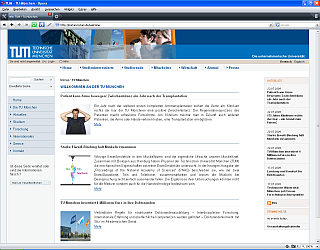
\includegraphics[height=2cm]{tumweb1.png}
\caption{Abbildungsbeispiel}\label{abbbeispiel}}
\end{figure}

\subsection{Listen}

Listen und Aufz"ahlungen sind wie gewohnt zu Verwenden. Nummerierungen werden dabei
ein St"uck (0,5~Zoll) einger"uckt.

\subsection{Fu"snoten}

Fu"snoten werden wie gewohnt mit \slcmd{footnote} eingegeben. Sie
erscheinen automatisch am unteren Ende der Seite und werden kapitelweise durchnummeriert.

\subsection{Und der ganze Rest?}

Die normalen \LaTeX{}-Kommandos wurden nicht ver"andert und deswegen hier auch nicht
beschrieben. Dazu geh"oren auch wie im folgenden Beispiel Formeln:

\[
\cos\frac{\alpha}{\sqrt{2}}t\cos{}h\frac{\alpha}{\sqrt{2}}t
\]

Das Setzen von Formeln und Tabellen erfolgt in der gewohnten Weise. F"ur Formeln
wird dabei auf die entsprechende \LaTeX{}-Standardschrift zur"uckgegriffen, da die
TUM Neue Helvetica nicht alle Zeichen kennt, die f"ur den Formelsatz n"otig w"are.

\begin{table}[H]\center{
\begin{tabular}{|l|r|}
\hline
\multicolumn{2}{|c|}{Zeitplan}\\ \hline
Besprechung & 8:20 \\ \hline
Kaffeepause & 10:00 \\ \hline
\end{tabular}
\caption{Beispieltabelle}\label{beispieltabelle}}
\end{table}


Sollte ein Befehl doch nicht so funktionieren wie erwartet und beschrieben, so schreiben
Sie bitte an \href{mailto:tum@as-computer.de}{tum@as-computer.de}.

\section{Bibliographie}

Zur Erstellung der Bibliographie wird Bibtex eingesetzt. Vorgesehen ist hierf"ur der Einsatz von \fn{tumbib.bst}. Dieser benutzt das Paket \cmd{harvard}, das auf die sonst "ublichen eckigen Klammern der \LaTeX{}-Bibliographien verzichtet.

Zitate im Text erfolgen entweder wie gewohnt mit \slcmd{cite} oder
mit den Harvard-Erweiterungen. Im speziellen ist es praktisch \slcmd{citeasnoun}
im Text zu nutzen, um damit auf die "uberfl"ussige Klammerung des Zitatursprungs zu
verzichten. Die Verwendung der entsprechenden Befehle kann man bei \citeasnoun{hfbs}
nachlesen.

Soll lieber eine andere Bibliographieanwendung verwendet werden, so l"asst sich
das \cmd{harvard}-Paket "uber die Option \cmd{standardbib} f"ur das Dokument
ausschalten.

\chapter{Installation}
\label{install}

Um die hier beschriebenen Schritte ausf"uhren zu k"onnen, m"ussen Sie meist Administratorrechte haben.


\chapter{Automatische Installation f"ur \MiKTeX{}}

Dazu entpacken Sie bitte das Paket \fn{tum-miktex.zip} und starten Sie das Programm \fn{tum-miktex-install.cmd}. Auf Windows Vista m"ussen Sie das Programm als Administrator starten.

Die Installation wurde mit \MiKTeX{}~2.7 getestet. Bei Problemen oder Fragen
wenden Sie sich bitte an Ihren Systemadministrator oder an \maintainers{}.


\chapter{Manuelle Installation f"ur Linux, Cygwin}

\section{Lokales Installationsverzeichnis w"ahlen}
\label{chooselocation}

Empfohlen: \quad{} \fn{/usr/local/share/texmf}

Dieses Verzeichnis wird von g"angigen Linuxdistributionen und in Cygwin automatisch erkannt.

\section{Archiv entpacken}

Beim Entpacken des Archivs \fn{tum-texmf.tgz} wird das Verzeichnis \fn{texmf} automatisch angelegt. Im obigen Beispiel entpacken Sie das Archiv also in \fn{/usr/local/share/} mit dem Kommando:

\begin{verbatim}
# cd /usr/local/share
# tar xzf tum-texmf.tgz
\end{verbatim}

\section{Schriftarten registrieren}

Bitte starten Sie in der Shell den Befehl

\begin{verbatim}
# updmap --enable Map tumhelv.map
\end{verbatim}

\chapter{Und los geht's!}

Am besten beginnen Sie damit, aus dem Verzeichnis \fn{texmf/tex/latex/tum/samples}
eine der Dateien \fn{brief.tex}, \fn{fax.tex} oder \fn{arbeit.tex} zu kopieren und auszuf"ullen. Das Verzeichnis \fn{texmf} finden Sie:

Bei \MiKTeX{}: Im Installationsverzeichnis, z.\,B. unter \fn{C:\bs{}Program Files(x86)\bs{}MiKTeX~2.7}.

Bei Linux: In dem in Abschnitt~\ref{chooselocation} gew"ahlten Verzeichnis.

Bitte beachten Sie, dass alle Vorlagen nur mit \cmd{pdflatex} funktionieren. Dabei werden die Hausschriften eingebettet und Web- oder Email-Adressen werden automatisch zu Hyperlinks.

\chapter{H"aufige Fragen}

\section{Der \LaTeX{}-Aufruf bringt eine Fehlermeldung}

\begin{verbatim}
! LaTeX Error: Cannot determine size of graphic in tumlogo.pdf (no BoundingBox)
\end{verbatim}

Bitte verwenden Sie \cmd{pdflatex}. Daf"ur werden die Hausschriften eingebettet und Web- oder Email-Adressen werden automatisch zu Hyperlinks.

Gelegentlich hilft es, alle generierten Dateien (\fn{*.aux}, \fn{*.toc},\,...) zu l"oschen und erneut \cmd{pdflatex} aufzurufen.

\section{Das Skript \fn{tum-miktex-install.cmd} gibt einen Fehler aus}

Bitte wenden Sie sich an \maintainers{}. Wenn m"oglich, h"angen Sie bitte die Fehlerausgabe an und nennen Sie uns Ihr Betriebssystem.
Falls Sie das Paket auf Windows Vista installieren m"ochten, beachten Sie, dass Sie das Installationsprogramm als Administrator starten m"ussen.

Als "Ubergangsl"osung k"onnten Sie die folgenden Schritte von Hand ausf"uhren und dabei eventuell feststellen, was genau schiefgegangen ist:

\begin{itemize}
\item Die Schriftzuordnungsdatei in die Konfiguration eintragen:
\begin{itemize}
    \item "Offnen Sie ein Kommandozeilenfenster (\cmd{Start \subnav{} Run\,... \subnav{} cmd})
    \item Geben Sie den Befehl \fn{initexmf -{}-edit-config-file=updmap.cfg} ein: \MiKTeX{} "offnet jetzt die richtige Konfigurationsdatei in einem Texteditor.
    \item F"ugen Sie der Datei am Ende die Zeile \cmd{Map tumhelv.map} hinzu
    \item Speichern Sie die Datei und schlie"sen Sie den Editor.
\end{itemize}
\item Das Paket installieren:
\begin{itemize}
    \item "Offnen Sie das \MiKTeX{}-Einstellungsprogramm: \cmd{Start \subnav{} Programme \subnav{} MiKTeX~2.7 \subnav{} Settings}
    \item Wechseln Sie zum Reiter \cmd{Packages}
    \item W"ahlen Sie das Repository: Klicken Sie auf \cmd{"Andern\,...}, w"ahlen Sie \cmd{Von Lokalem Verzeichnis}, w"ahlen Sie das Verzeichnis \cmd{package-repository} aus dem Installationspaket aus.
    \item Starten Sie den \cmd{Package Manager} durch klick auf den Button weiter unten im Dialogfenster.
    \item Um das richtige Paket schneller zu finden, geben Sie im Feld \cmd{Name:} den Namen \fn{tum} ein und dr"ucken Sie auf \cmd{Filter}.
    \item Markieren Sie das Paket \fn{tum} und klicken Sie auf das gro"se blaue Pluszeichen in der linken oberen Ecke des Fensters, um das Paket zu installieren.
    \item Schlie"sen Sie alle Dialoge und machen Sie einen Versuch mit einer der Beispieldateien, z.\,B. mit dem \fn{texmf/tex/latex/tum/samples/brief.tex}.
\end{itemize}
\item Eigentlich sollte das gen"ugen -- falls nun Ihre Dateien weitgehend verarbeitet werden aber die Schrift immer noch nicht gefunden wird, m"ussen Sie die Dateidatenbank aktualisieren:
\begin{itemize}
    \item Geben Sie in der Kommandozeile den Befehl \fn{initexmf -u -{}-mkmaps} ein: \MiKTeX{} durchsucht jetzt alle Installationsverzeichnisse und aktualisiert die notwendigen Datenbanken.
\end{itemize}
\end{itemize}


\section{Das Vorlagenpaket oder \MiKTeX{} lassen sich unter Vista nicht installieren}

Wir empfehlen folgende Einstellungen, damit die Installation gelingt:

\begin{itemize}
\item "Offnen Sie die Eigenschaften der Installationsdatei: Rechtsklick auf die Datei \fn{basic-miktex-...exe} bzw. \fn{tum-miktex-install.cmd}, ganz unten im Kontextmen"u finden Sie die \cmd{Eigenschaften}
\item Wechseln Sie zum Reiter \cmd{Kompatibilit"at}. Dort aktivieren Sie zun"achst \cmd{Kompatibilit"at zu Windows XP}
\item Weiter unten setzen Sie ein H"akchen bei \cmd{Als Administrator ausf"uhren}
\item Falls das H"akchen nicht aktiv ist, k"onnen Sie die Datei sp"ater auch anders mit Administratorrechten aufrufen (siehe unten) -- schlie"sen Sie zun"achst diesen Dialog
\item Starten Sie die Datei, gegebenenfalls "offnen Sie dazu das Kontextmen"u und w"ahlen \cmd{Als Administrator ausf"uhren}.
\end{itemize}


\section{Can I have these instructions in English, please?}

Tell us: \maintainers{}, we'll see what we can do.

\section{I would like to use letter or legal paper instead of DIN A4}

Other paper sizes than A4 are not defined by the corporate design. In Adobe reader, it should be easy to say ``Shrink to fit printable area''.

\section{Ich m"ochte die Vorlagen auf dem System XY verwenden}

Bitte teilen Sie uns das mit. Wir haben uns absichtlich auf eine "uberschaubare Anzahl von Zielplattformen beschr"ankt, um diese korrekt zu unterst"utzen. Vielleicht k"onnen wir Ihnen trotzdem auch bei einem anderen System helfen.

\section{Gibt es Formeln, Tabellen, andere Schriftarten, Sonderzeichen\,...\,?}

Es ist so, dass die Vorgaben des Corporate Designs sich auf bestimmte Aspekte, wie Schriftart und -gr"o"se, beschr"anken. Arbeiten Sie mit dem Dokument wie sie es sonst auch mit \LaTeX{} tun w"urden, und beachten Sie gelegentlich die Hinweise auf \tumcdurl{}, insbesondere \citeasnoun{tumcd}.

Falls Ihnen etwas wichtiges fehlt, sagen Sie uns bitte bescheid: \maintainers{}.

\clearpage
\appendix
\listoffigures
\listoftables
%%tex
%% $Id: anleitung.tex 74 2009-07-30 18:39:03Z miracle $
\documentclass[ngerman,12pt]{tumbook}
\usepackage{subfigure}
\usepackage{float}

%\raster

\makeindex
\newcommand{\bs}{\textbackslash}
\newcommand{\fn}[1]{,,\textsl{#1}``}
\newcommand{\cmd}[1]{\textbf{#1}}
\newcommand{\slcmd}[1]{\cmd{\textbackslash#1}}

\newcommand{\MiKTeX}{MiK\TeX{}}
\newcommand{\TeXLive}{\TeX{}Live}
\newcommand{\email}[1]{\textbf{\textsl{#1}}}
\newcommand{\maintainers}{\email{tum@as-computer.de}}
\newcommand{\ediseppmail}{\email{tum@ediundsepp.de}}
\newcommand{\tumcdurl}{http://www.tumcd.de/}
\newcommand{\subnav}{\guillemotright}

\Semester{WS 2009/2010}
\title{Arbeiten mit den TU-\LaTeX{}-Vorlagen}
\Untertitel{Eine kurze Anleitung zum Umgang mit tumbook.cls\\zur Erstellung von wissenschaftlichen Arbeiten f\"ur die TU M\"unchen}
\Themensteller{\textsl{ediundsepp} GbR Gestaltungsgesellschaft, M�nchen}
\TUMAdresse{}
\Autorenadresse{AS Computer Consulting \& Service GmbH, M\"unchen}
\Abgabetermin{31. Juli 2009}
\author{Ulrike Schrepf und Jan Schormann}
\date{M\"unchen, den \today}
\begin{document}
\maketitle
\tableofcontents

\clearpage

\chapter{Einleitung}

Dies ist ein Paket von Schriftartdateien und \LaTeX{}-Klassen,
die zusammen das Erstellen von Briefen und Faxnachrichten im Corporate Design
der Technischen Universit"at M"unchen erlauben.

\vspace{\baselineskip}

Das Corporate Design ist hier beschrieben: \tumcdurl{} \\
Bei Fragen zur Gestaltung: \ediseppmail{} \\
Bei Fragen zu den \LaTeX{}-Dokumenten oder zur Installation: \maintainers{}

Die Anleitung zur Installation finden Sie in Abschnitt~\ref{install} am Schluss dieses Dokuments.

\chapter{Grundlagen}

Bei \fn{tumbook.cls} handelt es sich um eine Abwandlung der bekannten
Dokumentklasse \fn{book.cls}. Die grundlegenden Bestandteile dieser Klasse blieben
dabei erhalten. Einige Optionen wurden allerdings durch fixe Vorgaben ersetzt
und weitere f"ur wissenschaftliche Arbeiten bei der TU typische Angaben wurden
in den Variablensatz "ubernommen.

Beim Arbeiten mit \fn{tumbook.cls} kann man also weitgehend die
Features der book-Dokumentklasse nutzen.

Einige Features der Bookklasse wurden mit Absicht ausgestellt. Dabei handelt
es sich um:
\begin{enumerate}
\item die Papierwahl -- nun voreingestellt auf DIN~A4.
\item die Titelseite -- nun immer auf einem eigenen Blatt.
\item die Kopfzeilen -- nun immer mit Seitenzahl in der Mitte.
\end{enumerate}

\section{Integrierte Pakete}

Folgende Pakete wurden in f"ur die Dokumentklasse bereits importiert, und lassen
sich damit ohne expliziten Eigenimport direkt nutzen:

\cmd{babel}\quad
\cmd{calc}\quad
\cmd{color}\quad
\cmd{epsfig}\quad
\cmd{float}\quad
\cmd{inputenc}

\chapter{Dokumenterstellung}

F"ur die Erstellung von Dokumenten f"ur die TU M"unchen werden einige spezielle
Anpassungen ben"otigt. Weitgehend wurde aber versucht auf die Standardkommandos
von \LaTeX{} zur"uckzugreifen, um erfahrenen \LaTeX{}-Benutzern die Arbeit
zu erleichtern und Einarbeitungszeiten zu verk"urzen.

\section{Vorarbeiten}

Einige der relevanten Informationen zu Dokument und Verarbeitung werden "uber
Optionen gesetzt oder in der Pr"aambel vereinbart. In diesem Abschnitt finden
Sie eine Liste dieser Optionen und Daten.

\subsection{Optionen}

Folgende Optionen sollten bei der Dokumentklasse gesetzt werden. Abh"angig von den
eingesetzten Paketen sind weitere Optionen m"oglich.

\begin{table}[H]
\center{
\begin{tabular}{|l|p{.32\textwidth}|p{.28\textwidth}|p{.13\textwidth}|}
\hline
\multicolumn{4}{|c|}{Optionsliste}\\ \hline
\textbf{Name/Art} & \textbf{Beschreibung}  & \textbf{m"ogliche Werte} & \textbf{Standard} \\  \hline
Encoding & \raggedright Im Text verwendete Zeichen; passend zu dieser Angabe werden Sonderzeichen interpretiert.
& \cmd{latin1, latin2, utf8,} \dots & --- \\ \hline
Sprache & \raggedright Spracheinstellung f"ur das Babel-Paket. & \raggedright \cmd{ngerman, english,} \dots & ---\\ \hline
Fakult"at & \raggedright Fakult"at f"ur die die Arbeit erstellt wurde;  bestimmt das Logo &
\raggedright \cmd{NEUTRAL, AR, BV, CH, EI, IN, MW, MA, MED, PH, SE, SP, WI, WZW} & \cmd{NEUTRAL} (kein Logo)\\ \hline
Schriftgr"o"se & \raggedright In der Arbeit verwendete Schriftgr"o"se & \cmd{9pt, 10pt, 12pt} & \cmd{10pt} \\ \hline
\end{tabular}}
\caption{Optionen f"ur die Dokumentklasse}
\end{table}

\subsection{Die Pr"aambel}

Folgende Daten sollten in der Pr"aambel gesetzt werden:

\begin{table}[H]
\center{
\begin{tabular}{|l|p{.55\textwidth}|c|}
\hline
\multicolumn{3}{|c|}{Pr"aambeldaten}\\ \hline
\textbf{Name} & \textbf{Beschreibung} & \textbf{obligatorisch} \\ \hline
\cmd{Seminar} & Seminartitel zur Arbeit & --- \\ \hline
\cmd{Semester} & Semester f"ur das die Arbeit geschrieben wurde & --- \\ \hline
\cmd{title} & Titel der Arbeit & x \\ \hline
\cmd{Untertitel} & Untertitel zur Arbeit & ---\\ \hline
\cmd{Themensteller} & Verantwortlicher Dozent & --- \\ \hline
\cmd{Autorenadresse} & Anschrift des Autors der Arbeit & --- \\ \hline
\cmd{Abgabetermin} & Verpflichtender Termin zur Abgabe & ---\\ \hline
\cmd{author} & Autor der Arbeit& x\\ \hline
\cmd{date} & Ort und Datum der Erstellung,
wird auch f"ur ehrenw"ortliche Erkl"arung eingesetzt & x \\ \hline
\cmd{Matrikelnummer} & Matrikelnummer des Autors
(ggf. mittels \LaTeX\-Befehlen gegliedert z.B. \slcmd{,}) & ---\\ \hline
\cmd{Fachsemester} & Fachsemester des Autors passend zum
angegebenen Semester oben & --- \\ \hline
\end{tabular}}
\caption{Informationen in der Pr"aambel}
\end{table}

\section{Aufbau des Dokuments}
Hier folgt eine Liste der Anpassungen, die zur Erstellung eines \textit{tumbooks} notwendig
sind. Die Bereiche des Dokuments entsprechen weitesgehend der Dokumentklasse \fn{book.cls}.

\subsection{Titelblatt}

Das Titelblatt wird wie gewohnt mit \slcmd{maketitle} erzeugt.
Das Titelblatt bekommt immer eine eigene Seite. Anders als bei \fn{book.cls}
gibt es bei \fn{tumbook.cls} keine Option \cmd{titlepage}.

Auf der Titelseite wird das Logo der TU und das Logo der Fakult"at angezeigt, wenn diese
"uber die Optionen korrekt ausgew"ahlt wurde.

\begin{figure}[H]
\center{
\subfigure{
\label{archlogo}
    
\epsfig{file=AR.pdf,height=9.605mm}
}
\subfigure{
    
\epsfig{file=BV.pdf,height=9.605mm}
}
\subfigure{
    
\epsfig{file=CH.pdf,height=9.605mm}
}
\subfigure{
    
\epsfig{file=EI.pdf,height=9.605mm}
}
\subfigure{
    
\epsfig{file=IN.pdf,height=9.605mm}
}
\subfigure{
   
\epsfig{file=MW.pdf,height=10.1mm,viewport=2.3mm 0mm 13.6mm 11mm}
}
\subfigure{
    
\epsfig{file=MA.pdf,height=9.605mm}
}
\subfigure{
    
\epsfig{file=MED.pdf,width=9.605mm,viewport=0mm 2.7mm 10.5mm 13.4mm}
}
\subfigure{
    
\epsfig{file=PH.pdf,height=9.605mm}
}
\subfigure{
    
\epsfig{file=SE.pdf,height=9.605mm}
}
\subfigure{
    
\epsfig{file=SP.pdf,height=10.065mm,viewport=2mm 0mm 13.4mm 11mm}
}
\subfigure{
    
\epsfig{file=WI.pdf,height=9.605mm,viewport=0.65mm 0mm 10.9mm 10.5mm}
}
\subfigure{
    
\epsfig{file=WZW.pdf,height=9.605mm}
}
\caption{Logos der TU M"unchen}\label{logos}}
\end{figure}


\subsection{"Uberschriften}

Innerhalb des Dokuments werden die "Uberschriftsebenen "uber \slcmd{chapter},
\slcmd{section}, \slcmd{subsection}, \slcmd{subsubsection} strukturiert.
Alle vier "Uberschriftsebenen werden im Inhaltsverzeichnis sichtbar.

Die Schriftgr"o"sen sind dabei entsprechend des Styleguides
bei allen "Uberschriften identisch und entsprechen der in den Optionen angegebenen
Schriftgr"o"se. Die verwendete Schrift ist TUM Neue Helvetica sowohl f"ur die normale im Dokument
verwendete Schrift als auch f"ur ausdr"uckliche Verwendung serifenloser Schrift.
Als nichtproportionale Schrift wird auf die entsprechende CMR-Schrift zur"uckgegriffen und
das Setzen von Formeln erfolgt ebenfalls nach dem \LaTeX{}-Standard.

\subsection{Verzeichnisse}

Inhaltsverzeichnis, Index, Abbildungs- und Tabellenverzeichnis werden wie bei den
Standard \LaTeX{}-Dokumenten erzeugt.

Einzig bei der Bibliographie kann der Stil \fn{tumbib.bst} eingesetzt werden\footnote{
s.~\citeasnoun{ttb} zur Verwendung von BibTeX}.

\subsection{Ehrenw"ortliche Erkl"arung}

Die typische Ehrenw"ortliche Erkl"arung, die angibt, dass der Autor das Dokument ohne
unerlaubte Hilfsmittel erstellt hat kann "uber \slcmd{Ehrenwort}
eingef"ugt werden. Name und Datum ergeben sich dabei aus den Angaben von
\slcmd{author} und \slcmd{date} aus der Pr"aambel.

Die Position daf"ur kann vom Ersteller frei gew"ahlt werden. Auch ob diese Erkl"arung
auf einer eigenen Seite erscheint, oder auf einer existierenden Seite platziert wird
ist dem Ersteller "uberlassen.

\section{Spezielle Inhalte}

Einige der Standardbefehle wurden abge"andert, um dem Styleguide der TU zu entsprechen.

\subsection{Abbildungen}

Abbildungen werden wie gewohnt "uber die \cmd{figure}-Umgebung intergriert.
Bei Verwendung des \cmd{ngerman} oder \cmd{german}-Pakets werden Abbildungen
mit ,,\textbf{Abb.}~\#`` beschriftet.
Bei Verwendung von \cmd{english} dagegen mit ,,\textbf{Fig.}~\#``. Alle anderen
Sprachen verwenden das in der jeweiligen Babelkonfiguration festgelegte Pr"afix.

Die Liste der Abbildungen wird wie gewohnt mit \slcmd{listoffigures}
in das Dokument integriert.

\begin{figure}[H]
\center{
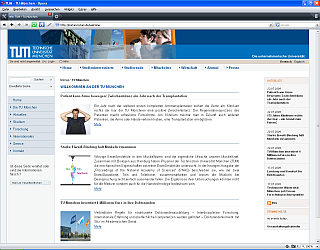
\includegraphics[height=2cm]{tumweb1.png}
\caption{Abbildungsbeispiel}\label{abbbeispiel}}
\end{figure}

\subsection{Listen}

Listen und Aufz"ahlungen sind wie gewohnt zu Verwenden. Nummerierungen werden dabei
ein St"uck (0,5~Zoll) einger"uckt.

\subsection{Fu"snoten}

Fu"snoten werden wie gewohnt mit \slcmd{footnote} eingegeben. Sie
erscheinen automatisch am unteren Ende der Seite und werden kapitelweise durchnummeriert.

\subsection{Und der ganze Rest?}

Die normalen \LaTeX{}-Kommandos wurden nicht ver"andert und deswegen hier auch nicht
beschrieben. Dazu geh"oren auch wie im folgenden Beispiel Formeln:

\[
\cos\frac{\alpha}{\sqrt{2}}t\cos{}h\frac{\alpha}{\sqrt{2}}t
\]

Das Setzen von Formeln und Tabellen erfolgt in der gewohnten Weise. F"ur Formeln
wird dabei auf die entsprechende \LaTeX{}-Standardschrift zur"uckgegriffen, da die
TUM Neue Helvetica nicht alle Zeichen kennt, die f"ur den Formelsatz n"otig w"are.

\begin{table}[H]\center{
\begin{tabular}{|l|r|}
\hline
\multicolumn{2}{|c|}{Zeitplan}\\ \hline
Besprechung & 8:20 \\ \hline
Kaffeepause & 10:00 \\ \hline
\end{tabular}
\caption{Beispieltabelle}\label{beispieltabelle}}
\end{table}


Sollte ein Befehl doch nicht so funktionieren wie erwartet und beschrieben, so schreiben
Sie bitte an \href{mailto:tum@as-computer.de}{tum@as-computer.de}.

\section{Bibliographie}

Zur Erstellung der Bibliographie wird Bibtex eingesetzt. Vorgesehen ist hierf"ur der Einsatz von \fn{tumbib.bst}. Dieser benutzt das Paket \cmd{harvard}, das auf die sonst "ublichen eckigen Klammern der \LaTeX{}-Bibliographien verzichtet.

Zitate im Text erfolgen entweder wie gewohnt mit \slcmd{cite} oder
mit den Harvard-Erweiterungen. Im speziellen ist es praktisch \slcmd{citeasnoun}
im Text zu nutzen, um damit auf die "uberfl"ussige Klammerung des Zitatursprungs zu
verzichten. Die Verwendung der entsprechenden Befehle kann man bei \citeasnoun{hfbs}
nachlesen.

Soll lieber eine andere Bibliographieanwendung verwendet werden, so l"asst sich
das \cmd{harvard}-Paket "uber die Option \cmd{standardbib} f"ur das Dokument
ausschalten.

\chapter{Installation}
\label{install}

Um die hier beschriebenen Schritte ausf"uhren zu k"onnen, m"ussen Sie meist Administratorrechte haben.


\chapter{Automatische Installation f"ur \MiKTeX{}}

Dazu entpacken Sie bitte das Paket \fn{tum-miktex.zip} und starten Sie das Programm \fn{tum-miktex-install.cmd}. Auf Windows Vista m"ussen Sie das Programm als Administrator starten.

Die Installation wurde mit \MiKTeX{}~2.7 getestet. Bei Problemen oder Fragen
wenden Sie sich bitte an Ihren Systemadministrator oder an \maintainers{}.


\chapter{Manuelle Installation f"ur Linux, Cygwin}

\section{Lokales Installationsverzeichnis w"ahlen}
\label{chooselocation}

Empfohlen: \quad{} \fn{/usr/local/share/texmf}

Dieses Verzeichnis wird von g"angigen Linuxdistributionen und in Cygwin automatisch erkannt.

\section{Archiv entpacken}

Beim Entpacken des Archivs \fn{tum-texmf.tgz} wird das Verzeichnis \fn{texmf} automatisch angelegt. Im obigen Beispiel entpacken Sie das Archiv also in \fn{/usr/local/share/} mit dem Kommando:

\begin{verbatim}
# cd /usr/local/share
# tar xzf tum-texmf.tgz
\end{verbatim}

\section{Schriftarten registrieren}

Bitte starten Sie in der Shell den Befehl

\begin{verbatim}
# updmap --enable Map tumhelv.map
\end{verbatim}

\chapter{Und los geht's!}

Am besten beginnen Sie damit, aus dem Verzeichnis \fn{texmf/tex/latex/tum/samples}
eine der Dateien \fn{brief.tex}, \fn{fax.tex} oder \fn{arbeit.tex} zu kopieren und auszuf"ullen. Das Verzeichnis \fn{texmf} finden Sie:

Bei \MiKTeX{}: Im Installationsverzeichnis, z.\,B. unter \fn{C:\bs{}Program Files(x86)\bs{}MiKTeX~2.7}.

Bei Linux: In dem in Abschnitt~\ref{chooselocation} gew"ahlten Verzeichnis.

Bitte beachten Sie, dass alle Vorlagen nur mit \cmd{pdflatex} funktionieren. Dabei werden die Hausschriften eingebettet und Web- oder Email-Adressen werden automatisch zu Hyperlinks.

\chapter{H"aufige Fragen}

\section{Der \LaTeX{}-Aufruf bringt eine Fehlermeldung}

\begin{verbatim}
! LaTeX Error: Cannot determine size of graphic in tumlogo.pdf (no BoundingBox)
\end{verbatim}

Bitte verwenden Sie \cmd{pdflatex}. Daf"ur werden die Hausschriften eingebettet und Web- oder Email-Adressen werden automatisch zu Hyperlinks.

Gelegentlich hilft es, alle generierten Dateien (\fn{*.aux}, \fn{*.toc},\,...) zu l"oschen und erneut \cmd{pdflatex} aufzurufen.

\section{Das Skript \fn{tum-miktex-install.cmd} gibt einen Fehler aus}

Bitte wenden Sie sich an \maintainers{}. Wenn m"oglich, h"angen Sie bitte die Fehlerausgabe an und nennen Sie uns Ihr Betriebssystem.
Falls Sie das Paket auf Windows Vista installieren m"ochten, beachten Sie, dass Sie das Installationsprogramm als Administrator starten m"ussen.

Als "Ubergangsl"osung k"onnten Sie die folgenden Schritte von Hand ausf"uhren und dabei eventuell feststellen, was genau schiefgegangen ist:

\begin{itemize}
\item Die Schriftzuordnungsdatei in die Konfiguration eintragen:
\begin{itemize}
    \item "Offnen Sie ein Kommandozeilenfenster (\cmd{Start \subnav{} Run\,... \subnav{} cmd})
    \item Geben Sie den Befehl \fn{initexmf -{}-edit-config-file=updmap.cfg} ein: \MiKTeX{} "offnet jetzt die richtige Konfigurationsdatei in einem Texteditor.
    \item F"ugen Sie der Datei am Ende die Zeile \cmd{Map tumhelv.map} hinzu
    \item Speichern Sie die Datei und schlie"sen Sie den Editor.
\end{itemize}
\item Das Paket installieren:
\begin{itemize}
    \item "Offnen Sie das \MiKTeX{}-Einstellungsprogramm: \cmd{Start \subnav{} Programme \subnav{} MiKTeX~2.7 \subnav{} Settings}
    \item Wechseln Sie zum Reiter \cmd{Packages}
    \item W"ahlen Sie das Repository: Klicken Sie auf \cmd{"Andern\,...}, w"ahlen Sie \cmd{Von Lokalem Verzeichnis}, w"ahlen Sie das Verzeichnis \cmd{package-repository} aus dem Installationspaket aus.
    \item Starten Sie den \cmd{Package Manager} durch klick auf den Button weiter unten im Dialogfenster.
    \item Um das richtige Paket schneller zu finden, geben Sie im Feld \cmd{Name:} den Namen \fn{tum} ein und dr"ucken Sie auf \cmd{Filter}.
    \item Markieren Sie das Paket \fn{tum} und klicken Sie auf das gro"se blaue Pluszeichen in der linken oberen Ecke des Fensters, um das Paket zu installieren.
    \item Schlie"sen Sie alle Dialoge und machen Sie einen Versuch mit einer der Beispieldateien, z.\,B. mit dem \fn{texmf/tex/latex/tum/samples/brief.tex}.
\end{itemize}
\item Eigentlich sollte das gen"ugen -- falls nun Ihre Dateien weitgehend verarbeitet werden aber die Schrift immer noch nicht gefunden wird, m"ussen Sie die Dateidatenbank aktualisieren:
\begin{itemize}
    \item Geben Sie in der Kommandozeile den Befehl \fn{initexmf -u -{}-mkmaps} ein: \MiKTeX{} durchsucht jetzt alle Installationsverzeichnisse und aktualisiert die notwendigen Datenbanken.
\end{itemize}
\end{itemize}


\section{Das Vorlagenpaket oder \MiKTeX{} lassen sich unter Vista nicht installieren}

Wir empfehlen folgende Einstellungen, damit die Installation gelingt:

\begin{itemize}
\item "Offnen Sie die Eigenschaften der Installationsdatei: Rechtsklick auf die Datei \fn{basic-miktex-...exe} bzw. \fn{tum-miktex-install.cmd}, ganz unten im Kontextmen"u finden Sie die \cmd{Eigenschaften}
\item Wechseln Sie zum Reiter \cmd{Kompatibilit"at}. Dort aktivieren Sie zun"achst \cmd{Kompatibilit"at zu Windows XP}
\item Weiter unten setzen Sie ein H"akchen bei \cmd{Als Administrator ausf"uhren}
\item Falls das H"akchen nicht aktiv ist, k"onnen Sie die Datei sp"ater auch anders mit Administratorrechten aufrufen (siehe unten) -- schlie"sen Sie zun"achst diesen Dialog
\item Starten Sie die Datei, gegebenenfalls "offnen Sie dazu das Kontextmen"u und w"ahlen \cmd{Als Administrator ausf"uhren}.
\end{itemize}


\section{Can I have these instructions in English, please?}

Tell us: \maintainers{}, we'll see what we can do.

\section{I would like to use letter or legal paper instead of DIN A4}

Other paper sizes than A4 are not defined by the corporate design. In Adobe reader, it should be easy to say ``Shrink to fit printable area''.

\section{Ich m"ochte die Vorlagen auf dem System XY verwenden}

Bitte teilen Sie uns das mit. Wir haben uns absichtlich auf eine "uberschaubare Anzahl von Zielplattformen beschr"ankt, um diese korrekt zu unterst"utzen. Vielleicht k"onnen wir Ihnen trotzdem auch bei einem anderen System helfen.

\section{Gibt es Formeln, Tabellen, andere Schriftarten, Sonderzeichen\,...\,?}

Es ist so, dass die Vorgaben des Corporate Designs sich auf bestimmte Aspekte, wie Schriftart und -gr"o"se, beschr"anken. Arbeiten Sie mit dem Dokument wie sie es sonst auch mit \LaTeX{} tun w"urden, und beachten Sie gelegentlich die Hinweise auf \tumcdurl{}, insbesondere \citeasnoun{tumcd}.

Falls Ihnen etwas wichtiges fehlt, sagen Sie uns bitte bescheid: \maintainers{}.

\clearpage
\appendix
\listoffigures
\listoftables
%%tex
%% $Id: anleitung.tex 74 2009-07-30 18:39:03Z miracle $
\documentclass[ngerman,12pt]{tumbook}
\usepackage{subfigure}
\usepackage{float}

%\raster

\makeindex
\newcommand{\bs}{\textbackslash}
\newcommand{\fn}[1]{,,\textsl{#1}``}
\newcommand{\cmd}[1]{\textbf{#1}}
\newcommand{\slcmd}[1]{\cmd{\textbackslash#1}}

\newcommand{\MiKTeX}{MiK\TeX{}}
\newcommand{\TeXLive}{\TeX{}Live}
\newcommand{\email}[1]{\textbf{\textsl{#1}}}
\newcommand{\maintainers}{\email{tum@as-computer.de}}
\newcommand{\ediseppmail}{\email{tum@ediundsepp.de}}
\newcommand{\tumcdurl}{http://www.tumcd.de/}
\newcommand{\subnav}{\guillemotright}

\Semester{WS 2009/2010}
\title{Arbeiten mit den TU-\LaTeX{}-Vorlagen}
\Untertitel{Eine kurze Anleitung zum Umgang mit tumbook.cls\\zur Erstellung von wissenschaftlichen Arbeiten f\"ur die TU M\"unchen}
\Themensteller{\textsl{ediundsepp} GbR Gestaltungsgesellschaft, M�nchen}
\TUMAdresse{}
\Autorenadresse{AS Computer Consulting \& Service GmbH, M\"unchen}
\Abgabetermin{31. Juli 2009}
\author{Ulrike Schrepf und Jan Schormann}
\date{M\"unchen, den \today}
\begin{document}
\maketitle
\tableofcontents

\clearpage

\chapter{Einleitung}

Dies ist ein Paket von Schriftartdateien und \LaTeX{}-Klassen,
die zusammen das Erstellen von Briefen und Faxnachrichten im Corporate Design
der Technischen Universit"at M"unchen erlauben.

\vspace{\baselineskip}

Das Corporate Design ist hier beschrieben: \tumcdurl{} \\
Bei Fragen zur Gestaltung: \ediseppmail{} \\
Bei Fragen zu den \LaTeX{}-Dokumenten oder zur Installation: \maintainers{}

Die Anleitung zur Installation finden Sie in Abschnitt~\ref{install} am Schluss dieses Dokuments.

\chapter{Grundlagen}

Bei \fn{tumbook.cls} handelt es sich um eine Abwandlung der bekannten
Dokumentklasse \fn{book.cls}. Die grundlegenden Bestandteile dieser Klasse blieben
dabei erhalten. Einige Optionen wurden allerdings durch fixe Vorgaben ersetzt
und weitere f"ur wissenschaftliche Arbeiten bei der TU typische Angaben wurden
in den Variablensatz "ubernommen.

Beim Arbeiten mit \fn{tumbook.cls} kann man also weitgehend die
Features der book-Dokumentklasse nutzen.

Einige Features der Bookklasse wurden mit Absicht ausgestellt. Dabei handelt
es sich um:
\begin{enumerate}
\item die Papierwahl -- nun voreingestellt auf DIN~A4.
\item die Titelseite -- nun immer auf einem eigenen Blatt.
\item die Kopfzeilen -- nun immer mit Seitenzahl in der Mitte.
\end{enumerate}

\section{Integrierte Pakete}

Folgende Pakete wurden in f"ur die Dokumentklasse bereits importiert, und lassen
sich damit ohne expliziten Eigenimport direkt nutzen:

\cmd{babel}\quad
\cmd{calc}\quad
\cmd{color}\quad
\cmd{epsfig}\quad
\cmd{float}\quad
\cmd{inputenc}

\chapter{Dokumenterstellung}

F"ur die Erstellung von Dokumenten f"ur die TU M"unchen werden einige spezielle
Anpassungen ben"otigt. Weitgehend wurde aber versucht auf die Standardkommandos
von \LaTeX{} zur"uckzugreifen, um erfahrenen \LaTeX{}-Benutzern die Arbeit
zu erleichtern und Einarbeitungszeiten zu verk"urzen.

\section{Vorarbeiten}

Einige der relevanten Informationen zu Dokument und Verarbeitung werden "uber
Optionen gesetzt oder in der Pr"aambel vereinbart. In diesem Abschnitt finden
Sie eine Liste dieser Optionen und Daten.

\subsection{Optionen}

Folgende Optionen sollten bei der Dokumentklasse gesetzt werden. Abh"angig von den
eingesetzten Paketen sind weitere Optionen m"oglich.

\begin{table}[H]
\center{
\begin{tabular}{|l|p{.32\textwidth}|p{.28\textwidth}|p{.13\textwidth}|}
\hline
\multicolumn{4}{|c|}{Optionsliste}\\ \hline
\textbf{Name/Art} & \textbf{Beschreibung}  & \textbf{m"ogliche Werte} & \textbf{Standard} \\  \hline
Encoding & \raggedright Im Text verwendete Zeichen; passend zu dieser Angabe werden Sonderzeichen interpretiert.
& \cmd{latin1, latin2, utf8,} \dots & --- \\ \hline
Sprache & \raggedright Spracheinstellung f"ur das Babel-Paket. & \raggedright \cmd{ngerman, english,} \dots & ---\\ \hline
Fakult"at & \raggedright Fakult"at f"ur die die Arbeit erstellt wurde;  bestimmt das Logo &
\raggedright \cmd{NEUTRAL, AR, BV, CH, EI, IN, MW, MA, MED, PH, SE, SP, WI, WZW} & \cmd{NEUTRAL} (kein Logo)\\ \hline
Schriftgr"o"se & \raggedright In der Arbeit verwendete Schriftgr"o"se & \cmd{9pt, 10pt, 12pt} & \cmd{10pt} \\ \hline
\end{tabular}}
\caption{Optionen f"ur die Dokumentklasse}
\end{table}

\subsection{Die Pr"aambel}

Folgende Daten sollten in der Pr"aambel gesetzt werden:

\begin{table}[H]
\center{
\begin{tabular}{|l|p{.55\textwidth}|c|}
\hline
\multicolumn{3}{|c|}{Pr"aambeldaten}\\ \hline
\textbf{Name} & \textbf{Beschreibung} & \textbf{obligatorisch} \\ \hline
\cmd{Seminar} & Seminartitel zur Arbeit & --- \\ \hline
\cmd{Semester} & Semester f"ur das die Arbeit geschrieben wurde & --- \\ \hline
\cmd{title} & Titel der Arbeit & x \\ \hline
\cmd{Untertitel} & Untertitel zur Arbeit & ---\\ \hline
\cmd{Themensteller} & Verantwortlicher Dozent & --- \\ \hline
\cmd{Autorenadresse} & Anschrift des Autors der Arbeit & --- \\ \hline
\cmd{Abgabetermin} & Verpflichtender Termin zur Abgabe & ---\\ \hline
\cmd{author} & Autor der Arbeit& x\\ \hline
\cmd{date} & Ort und Datum der Erstellung,
wird auch f"ur ehrenw"ortliche Erkl"arung eingesetzt & x \\ \hline
\cmd{Matrikelnummer} & Matrikelnummer des Autors
(ggf. mittels \LaTeX\-Befehlen gegliedert z.B. \slcmd{,}) & ---\\ \hline
\cmd{Fachsemester} & Fachsemester des Autors passend zum
angegebenen Semester oben & --- \\ \hline
\end{tabular}}
\caption{Informationen in der Pr"aambel}
\end{table}

\section{Aufbau des Dokuments}
Hier folgt eine Liste der Anpassungen, die zur Erstellung eines \textit{tumbooks} notwendig
sind. Die Bereiche des Dokuments entsprechen weitesgehend der Dokumentklasse \fn{book.cls}.

\subsection{Titelblatt}

Das Titelblatt wird wie gewohnt mit \slcmd{maketitle} erzeugt.
Das Titelblatt bekommt immer eine eigene Seite. Anders als bei \fn{book.cls}
gibt es bei \fn{tumbook.cls} keine Option \cmd{titlepage}.

Auf der Titelseite wird das Logo der TU und das Logo der Fakult"at angezeigt, wenn diese
"uber die Optionen korrekt ausgew"ahlt wurde.

\begin{figure}[H]
\center{
\subfigure{
\label{archlogo}
    
\epsfig{file=AR.pdf,height=9.605mm}
}
\subfigure{
    
\epsfig{file=BV.pdf,height=9.605mm}
}
\subfigure{
    
\epsfig{file=CH.pdf,height=9.605mm}
}
\subfigure{
    
\epsfig{file=EI.pdf,height=9.605mm}
}
\subfigure{
    
\epsfig{file=IN.pdf,height=9.605mm}
}
\subfigure{
   
\epsfig{file=MW.pdf,height=10.1mm,viewport=2.3mm 0mm 13.6mm 11mm}
}
\subfigure{
    
\epsfig{file=MA.pdf,height=9.605mm}
}
\subfigure{
    
\epsfig{file=MED.pdf,width=9.605mm,viewport=0mm 2.7mm 10.5mm 13.4mm}
}
\subfigure{
    
\epsfig{file=PH.pdf,height=9.605mm}
}
\subfigure{
    
\epsfig{file=SE.pdf,height=9.605mm}
}
\subfigure{
    
\epsfig{file=SP.pdf,height=10.065mm,viewport=2mm 0mm 13.4mm 11mm}
}
\subfigure{
    
\epsfig{file=WI.pdf,height=9.605mm,viewport=0.65mm 0mm 10.9mm 10.5mm}
}
\subfigure{
    
\epsfig{file=WZW.pdf,height=9.605mm}
}
\caption{Logos der TU M"unchen}\label{logos}}
\end{figure}


\subsection{"Uberschriften}

Innerhalb des Dokuments werden die "Uberschriftsebenen "uber \slcmd{chapter},
\slcmd{section}, \slcmd{subsection}, \slcmd{subsubsection} strukturiert.
Alle vier "Uberschriftsebenen werden im Inhaltsverzeichnis sichtbar.

Die Schriftgr"o"sen sind dabei entsprechend des Styleguides
bei allen "Uberschriften identisch und entsprechen der in den Optionen angegebenen
Schriftgr"o"se. Die verwendete Schrift ist TUM Neue Helvetica sowohl f"ur die normale im Dokument
verwendete Schrift als auch f"ur ausdr"uckliche Verwendung serifenloser Schrift.
Als nichtproportionale Schrift wird auf die entsprechende CMR-Schrift zur"uckgegriffen und
das Setzen von Formeln erfolgt ebenfalls nach dem \LaTeX{}-Standard.

\subsection{Verzeichnisse}

Inhaltsverzeichnis, Index, Abbildungs- und Tabellenverzeichnis werden wie bei den
Standard \LaTeX{}-Dokumenten erzeugt.

Einzig bei der Bibliographie kann der Stil \fn{tumbib.bst} eingesetzt werden\footnote{
s.~\citeasnoun{ttb} zur Verwendung von BibTeX}.

\subsection{Ehrenw"ortliche Erkl"arung}

Die typische Ehrenw"ortliche Erkl"arung, die angibt, dass der Autor das Dokument ohne
unerlaubte Hilfsmittel erstellt hat kann "uber \slcmd{Ehrenwort}
eingef"ugt werden. Name und Datum ergeben sich dabei aus den Angaben von
\slcmd{author} und \slcmd{date} aus der Pr"aambel.

Die Position daf"ur kann vom Ersteller frei gew"ahlt werden. Auch ob diese Erkl"arung
auf einer eigenen Seite erscheint, oder auf einer existierenden Seite platziert wird
ist dem Ersteller "uberlassen.

\section{Spezielle Inhalte}

Einige der Standardbefehle wurden abge"andert, um dem Styleguide der TU zu entsprechen.

\subsection{Abbildungen}

Abbildungen werden wie gewohnt "uber die \cmd{figure}-Umgebung intergriert.
Bei Verwendung des \cmd{ngerman} oder \cmd{german}-Pakets werden Abbildungen
mit ,,\textbf{Abb.}~\#`` beschriftet.
Bei Verwendung von \cmd{english} dagegen mit ,,\textbf{Fig.}~\#``. Alle anderen
Sprachen verwenden das in der jeweiligen Babelkonfiguration festgelegte Pr"afix.

Die Liste der Abbildungen wird wie gewohnt mit \slcmd{listoffigures}
in das Dokument integriert.

\begin{figure}[H]
\center{
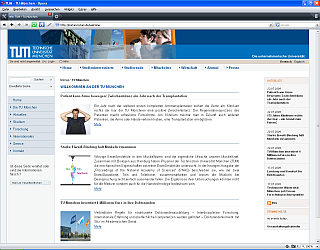
\includegraphics[height=2cm]{tumweb1.png}
\caption{Abbildungsbeispiel}\label{abbbeispiel}}
\end{figure}

\subsection{Listen}

Listen und Aufz"ahlungen sind wie gewohnt zu Verwenden. Nummerierungen werden dabei
ein St"uck (0,5~Zoll) einger"uckt.

\subsection{Fu"snoten}

Fu"snoten werden wie gewohnt mit \slcmd{footnote} eingegeben. Sie
erscheinen automatisch am unteren Ende der Seite und werden kapitelweise durchnummeriert.

\subsection{Und der ganze Rest?}

Die normalen \LaTeX{}-Kommandos wurden nicht ver"andert und deswegen hier auch nicht
beschrieben. Dazu geh"oren auch wie im folgenden Beispiel Formeln:

\[
\cos\frac{\alpha}{\sqrt{2}}t\cos{}h\frac{\alpha}{\sqrt{2}}t
\]

Das Setzen von Formeln und Tabellen erfolgt in der gewohnten Weise. F"ur Formeln
wird dabei auf die entsprechende \LaTeX{}-Standardschrift zur"uckgegriffen, da die
TUM Neue Helvetica nicht alle Zeichen kennt, die f"ur den Formelsatz n"otig w"are.

\begin{table}[H]\center{
\begin{tabular}{|l|r|}
\hline
\multicolumn{2}{|c|}{Zeitplan}\\ \hline
Besprechung & 8:20 \\ \hline
Kaffeepause & 10:00 \\ \hline
\end{tabular}
\caption{Beispieltabelle}\label{beispieltabelle}}
\end{table}


Sollte ein Befehl doch nicht so funktionieren wie erwartet und beschrieben, so schreiben
Sie bitte an \href{mailto:tum@as-computer.de}{tum@as-computer.de}.

\section{Bibliographie}

Zur Erstellung der Bibliographie wird Bibtex eingesetzt. Vorgesehen ist hierf"ur der Einsatz von \fn{tumbib.bst}. Dieser benutzt das Paket \cmd{harvard}, das auf die sonst "ublichen eckigen Klammern der \LaTeX{}-Bibliographien verzichtet.

Zitate im Text erfolgen entweder wie gewohnt mit \slcmd{cite} oder
mit den Harvard-Erweiterungen. Im speziellen ist es praktisch \slcmd{citeasnoun}
im Text zu nutzen, um damit auf die "uberfl"ussige Klammerung des Zitatursprungs zu
verzichten. Die Verwendung der entsprechenden Befehle kann man bei \citeasnoun{hfbs}
nachlesen.

Soll lieber eine andere Bibliographieanwendung verwendet werden, so l"asst sich
das \cmd{harvard}-Paket "uber die Option \cmd{standardbib} f"ur das Dokument
ausschalten.

\chapter{Installation}
\label{install}

Um die hier beschriebenen Schritte ausf"uhren zu k"onnen, m"ussen Sie meist Administratorrechte haben.


\chapter{Automatische Installation f"ur \MiKTeX{}}

Dazu entpacken Sie bitte das Paket \fn{tum-miktex.zip} und starten Sie das Programm \fn{tum-miktex-install.cmd}. Auf Windows Vista m"ussen Sie das Programm als Administrator starten.

Die Installation wurde mit \MiKTeX{}~2.7 getestet. Bei Problemen oder Fragen
wenden Sie sich bitte an Ihren Systemadministrator oder an \maintainers{}.


\chapter{Manuelle Installation f"ur Linux, Cygwin}

\section{Lokales Installationsverzeichnis w"ahlen}
\label{chooselocation}

Empfohlen: \quad{} \fn{/usr/local/share/texmf}

Dieses Verzeichnis wird von g"angigen Linuxdistributionen und in Cygwin automatisch erkannt.

\section{Archiv entpacken}

Beim Entpacken des Archivs \fn{tum-texmf.tgz} wird das Verzeichnis \fn{texmf} automatisch angelegt. Im obigen Beispiel entpacken Sie das Archiv also in \fn{/usr/local/share/} mit dem Kommando:

\begin{verbatim}
# cd /usr/local/share
# tar xzf tum-texmf.tgz
\end{verbatim}

\section{Schriftarten registrieren}

Bitte starten Sie in der Shell den Befehl

\begin{verbatim}
# updmap --enable Map tumhelv.map
\end{verbatim}

\chapter{Und los geht's!}

Am besten beginnen Sie damit, aus dem Verzeichnis \fn{texmf/tex/latex/tum/samples}
eine der Dateien \fn{brief.tex}, \fn{fax.tex} oder \fn{arbeit.tex} zu kopieren und auszuf"ullen. Das Verzeichnis \fn{texmf} finden Sie:

Bei \MiKTeX{}: Im Installationsverzeichnis, z.\,B. unter \fn{C:\bs{}Program Files(x86)\bs{}MiKTeX~2.7}.

Bei Linux: In dem in Abschnitt~\ref{chooselocation} gew"ahlten Verzeichnis.

Bitte beachten Sie, dass alle Vorlagen nur mit \cmd{pdflatex} funktionieren. Dabei werden die Hausschriften eingebettet und Web- oder Email-Adressen werden automatisch zu Hyperlinks.

\chapter{H"aufige Fragen}

\section{Der \LaTeX{}-Aufruf bringt eine Fehlermeldung}

\begin{verbatim}
! LaTeX Error: Cannot determine size of graphic in tumlogo.pdf (no BoundingBox)
\end{verbatim}

Bitte verwenden Sie \cmd{pdflatex}. Daf"ur werden die Hausschriften eingebettet und Web- oder Email-Adressen werden automatisch zu Hyperlinks.

Gelegentlich hilft es, alle generierten Dateien (\fn{*.aux}, \fn{*.toc},\,...) zu l"oschen und erneut \cmd{pdflatex} aufzurufen.

\section{Das Skript \fn{tum-miktex-install.cmd} gibt einen Fehler aus}

Bitte wenden Sie sich an \maintainers{}. Wenn m"oglich, h"angen Sie bitte die Fehlerausgabe an und nennen Sie uns Ihr Betriebssystem.
Falls Sie das Paket auf Windows Vista installieren m"ochten, beachten Sie, dass Sie das Installationsprogramm als Administrator starten m"ussen.

Als "Ubergangsl"osung k"onnten Sie die folgenden Schritte von Hand ausf"uhren und dabei eventuell feststellen, was genau schiefgegangen ist:

\begin{itemize}
\item Die Schriftzuordnungsdatei in die Konfiguration eintragen:
\begin{itemize}
    \item "Offnen Sie ein Kommandozeilenfenster (\cmd{Start \subnav{} Run\,... \subnav{} cmd})
    \item Geben Sie den Befehl \fn{initexmf -{}-edit-config-file=updmap.cfg} ein: \MiKTeX{} "offnet jetzt die richtige Konfigurationsdatei in einem Texteditor.
    \item F"ugen Sie der Datei am Ende die Zeile \cmd{Map tumhelv.map} hinzu
    \item Speichern Sie die Datei und schlie"sen Sie den Editor.
\end{itemize}
\item Das Paket installieren:
\begin{itemize}
    \item "Offnen Sie das \MiKTeX{}-Einstellungsprogramm: \cmd{Start \subnav{} Programme \subnav{} MiKTeX~2.7 \subnav{} Settings}
    \item Wechseln Sie zum Reiter \cmd{Packages}
    \item W"ahlen Sie das Repository: Klicken Sie auf \cmd{"Andern\,...}, w"ahlen Sie \cmd{Von Lokalem Verzeichnis}, w"ahlen Sie das Verzeichnis \cmd{package-repository} aus dem Installationspaket aus.
    \item Starten Sie den \cmd{Package Manager} durch klick auf den Button weiter unten im Dialogfenster.
    \item Um das richtige Paket schneller zu finden, geben Sie im Feld \cmd{Name:} den Namen \fn{tum} ein und dr"ucken Sie auf \cmd{Filter}.
    \item Markieren Sie das Paket \fn{tum} und klicken Sie auf das gro"se blaue Pluszeichen in der linken oberen Ecke des Fensters, um das Paket zu installieren.
    \item Schlie"sen Sie alle Dialoge und machen Sie einen Versuch mit einer der Beispieldateien, z.\,B. mit dem \fn{texmf/tex/latex/tum/samples/brief.tex}.
\end{itemize}
\item Eigentlich sollte das gen"ugen -- falls nun Ihre Dateien weitgehend verarbeitet werden aber die Schrift immer noch nicht gefunden wird, m"ussen Sie die Dateidatenbank aktualisieren:
\begin{itemize}
    \item Geben Sie in der Kommandozeile den Befehl \fn{initexmf -u -{}-mkmaps} ein: \MiKTeX{} durchsucht jetzt alle Installationsverzeichnisse und aktualisiert die notwendigen Datenbanken.
\end{itemize}
\end{itemize}


\section{Das Vorlagenpaket oder \MiKTeX{} lassen sich unter Vista nicht installieren}

Wir empfehlen folgende Einstellungen, damit die Installation gelingt:

\begin{itemize}
\item "Offnen Sie die Eigenschaften der Installationsdatei: Rechtsklick auf die Datei \fn{basic-miktex-...exe} bzw. \fn{tum-miktex-install.cmd}, ganz unten im Kontextmen"u finden Sie die \cmd{Eigenschaften}
\item Wechseln Sie zum Reiter \cmd{Kompatibilit"at}. Dort aktivieren Sie zun"achst \cmd{Kompatibilit"at zu Windows XP}
\item Weiter unten setzen Sie ein H"akchen bei \cmd{Als Administrator ausf"uhren}
\item Falls das H"akchen nicht aktiv ist, k"onnen Sie die Datei sp"ater auch anders mit Administratorrechten aufrufen (siehe unten) -- schlie"sen Sie zun"achst diesen Dialog
\item Starten Sie die Datei, gegebenenfalls "offnen Sie dazu das Kontextmen"u und w"ahlen \cmd{Als Administrator ausf"uhren}.
\end{itemize}


\section{Can I have these instructions in English, please?}

Tell us: \maintainers{}, we'll see what we can do.

\section{I would like to use letter or legal paper instead of DIN A4}

Other paper sizes than A4 are not defined by the corporate design. In Adobe reader, it should be easy to say ``Shrink to fit printable area''.

\section{Ich m"ochte die Vorlagen auf dem System XY verwenden}

Bitte teilen Sie uns das mit. Wir haben uns absichtlich auf eine "uberschaubare Anzahl von Zielplattformen beschr"ankt, um diese korrekt zu unterst"utzen. Vielleicht k"onnen wir Ihnen trotzdem auch bei einem anderen System helfen.

\section{Gibt es Formeln, Tabellen, andere Schriftarten, Sonderzeichen\,...\,?}

Es ist so, dass die Vorgaben des Corporate Designs sich auf bestimmte Aspekte, wie Schriftart und -gr"o"se, beschr"anken. Arbeiten Sie mit dem Dokument wie sie es sonst auch mit \LaTeX{} tun w"urden, und beachten Sie gelegentlich die Hinweise auf \tumcdurl{}, insbesondere \citeasnoun{tumcd}.

Falls Ihnen etwas wichtiges fehlt, sagen Sie uns bitte bescheid: \maintainers{}.

\clearpage
\appendix
\listoffigures
\listoftables
%%tex
%% $Id: anleitung.tex 74 2009-07-30 18:39:03Z miracle $
\documentclass[ngerman,12pt]{tumbook}
\usepackage{subfigure}
\usepackage{float}

%\raster

\makeindex
\newcommand{\bs}{\textbackslash}
\newcommand{\fn}[1]{,,\textsl{#1}``}
\newcommand{\cmd}[1]{\textbf{#1}}
\newcommand{\slcmd}[1]{\cmd{\textbackslash#1}}

\newcommand{\MiKTeX}{MiK\TeX{}}
\newcommand{\TeXLive}{\TeX{}Live}
\newcommand{\email}[1]{\textbf{\textsl{#1}}}
\newcommand{\maintainers}{\email{tum@as-computer.de}}
\newcommand{\ediseppmail}{\email{tum@ediundsepp.de}}
\newcommand{\tumcdurl}{http://www.tumcd.de/}
\newcommand{\subnav}{\guillemotright}

\Semester{WS 2009/2010}
\title{Arbeiten mit den TU-\LaTeX{}-Vorlagen}
\Untertitel{Eine kurze Anleitung zum Umgang mit tumbook.cls\\zur Erstellung von wissenschaftlichen Arbeiten f\"ur die TU M\"unchen}
\Themensteller{\textsl{ediundsepp} GbR Gestaltungsgesellschaft, M�nchen}
\TUMAdresse{}
\Autorenadresse{AS Computer Consulting \& Service GmbH, M\"unchen}
\Abgabetermin{31. Juli 2009}
\author{Ulrike Schrepf und Jan Schormann}
\date{M\"unchen, den \today}
\begin{document}
\maketitle
\tableofcontents

\clearpage

\chapter{Einleitung}

Dies ist ein Paket von Schriftartdateien und \LaTeX{}-Klassen,
die zusammen das Erstellen von Briefen und Faxnachrichten im Corporate Design
der Technischen Universit"at M"unchen erlauben.

\vspace{\baselineskip}

Das Corporate Design ist hier beschrieben: \tumcdurl{} \\
Bei Fragen zur Gestaltung: \ediseppmail{} \\
Bei Fragen zu den \LaTeX{}-Dokumenten oder zur Installation: \maintainers{}

Die Anleitung zur Installation finden Sie in Abschnitt~\ref{install} am Schluss dieses Dokuments.

\chapter{Grundlagen}

Bei \fn{tumbook.cls} handelt es sich um eine Abwandlung der bekannten
Dokumentklasse \fn{book.cls}. Die grundlegenden Bestandteile dieser Klasse blieben
dabei erhalten. Einige Optionen wurden allerdings durch fixe Vorgaben ersetzt
und weitere f"ur wissenschaftliche Arbeiten bei der TU typische Angaben wurden
in den Variablensatz "ubernommen.

Beim Arbeiten mit \fn{tumbook.cls} kann man also weitgehend die
Features der book-Dokumentklasse nutzen.

Einige Features der Bookklasse wurden mit Absicht ausgestellt. Dabei handelt
es sich um:
\begin{enumerate}
\item die Papierwahl -- nun voreingestellt auf DIN~A4.
\item die Titelseite -- nun immer auf einem eigenen Blatt.
\item die Kopfzeilen -- nun immer mit Seitenzahl in der Mitte.
\end{enumerate}

\section{Integrierte Pakete}

Folgende Pakete wurden in f"ur die Dokumentklasse bereits importiert, und lassen
sich damit ohne expliziten Eigenimport direkt nutzen:

\cmd{babel}\quad
\cmd{calc}\quad
\cmd{color}\quad
\cmd{epsfig}\quad
\cmd{float}\quad
\cmd{inputenc}

\chapter{Dokumenterstellung}

F"ur die Erstellung von Dokumenten f"ur die TU M"unchen werden einige spezielle
Anpassungen ben"otigt. Weitgehend wurde aber versucht auf die Standardkommandos
von \LaTeX{} zur"uckzugreifen, um erfahrenen \LaTeX{}-Benutzern die Arbeit
zu erleichtern und Einarbeitungszeiten zu verk"urzen.

\section{Vorarbeiten}

Einige der relevanten Informationen zu Dokument und Verarbeitung werden "uber
Optionen gesetzt oder in der Pr"aambel vereinbart. In diesem Abschnitt finden
Sie eine Liste dieser Optionen und Daten.

\subsection{Optionen}

Folgende Optionen sollten bei der Dokumentklasse gesetzt werden. Abh"angig von den
eingesetzten Paketen sind weitere Optionen m"oglich.

\begin{table}[H]
\center{
\begin{tabular}{|l|p{.32\textwidth}|p{.28\textwidth}|p{.13\textwidth}|}
\hline
\multicolumn{4}{|c|}{Optionsliste}\\ \hline
\textbf{Name/Art} & \textbf{Beschreibung}  & \textbf{m"ogliche Werte} & \textbf{Standard} \\  \hline
Encoding & \raggedright Im Text verwendete Zeichen; passend zu dieser Angabe werden Sonderzeichen interpretiert.
& \cmd{latin1, latin2, utf8,} \dots & --- \\ \hline
Sprache & \raggedright Spracheinstellung f"ur das Babel-Paket. & \raggedright \cmd{ngerman, english,} \dots & ---\\ \hline
Fakult"at & \raggedright Fakult"at f"ur die die Arbeit erstellt wurde;  bestimmt das Logo &
\raggedright \cmd{NEUTRAL, AR, BV, CH, EI, IN, MW, MA, MED, PH, SE, SP, WI, WZW} & \cmd{NEUTRAL} (kein Logo)\\ \hline
Schriftgr"o"se & \raggedright In der Arbeit verwendete Schriftgr"o"se & \cmd{9pt, 10pt, 12pt} & \cmd{10pt} \\ \hline
\end{tabular}}
\caption{Optionen f"ur die Dokumentklasse}
\end{table}

\subsection{Die Pr"aambel}

Folgende Daten sollten in der Pr"aambel gesetzt werden:

\begin{table}[H]
\center{
\begin{tabular}{|l|p{.55\textwidth}|c|}
\hline
\multicolumn{3}{|c|}{Pr"aambeldaten}\\ \hline
\textbf{Name} & \textbf{Beschreibung} & \textbf{obligatorisch} \\ \hline
\cmd{Seminar} & Seminartitel zur Arbeit & --- \\ \hline
\cmd{Semester} & Semester f"ur das die Arbeit geschrieben wurde & --- \\ \hline
\cmd{title} & Titel der Arbeit & x \\ \hline
\cmd{Untertitel} & Untertitel zur Arbeit & ---\\ \hline
\cmd{Themensteller} & Verantwortlicher Dozent & --- \\ \hline
\cmd{Autorenadresse} & Anschrift des Autors der Arbeit & --- \\ \hline
\cmd{Abgabetermin} & Verpflichtender Termin zur Abgabe & ---\\ \hline
\cmd{author} & Autor der Arbeit& x\\ \hline
\cmd{date} & Ort und Datum der Erstellung,
wird auch f"ur ehrenw"ortliche Erkl"arung eingesetzt & x \\ \hline
\cmd{Matrikelnummer} & Matrikelnummer des Autors
(ggf. mittels \LaTeX\-Befehlen gegliedert z.B. \slcmd{,}) & ---\\ \hline
\cmd{Fachsemester} & Fachsemester des Autors passend zum
angegebenen Semester oben & --- \\ \hline
\end{tabular}}
\caption{Informationen in der Pr"aambel}
\end{table}

\section{Aufbau des Dokuments}
Hier folgt eine Liste der Anpassungen, die zur Erstellung eines \textit{tumbooks} notwendig
sind. Die Bereiche des Dokuments entsprechen weitesgehend der Dokumentklasse \fn{book.cls}.

\subsection{Titelblatt}

Das Titelblatt wird wie gewohnt mit \slcmd{maketitle} erzeugt.
Das Titelblatt bekommt immer eine eigene Seite. Anders als bei \fn{book.cls}
gibt es bei \fn{tumbook.cls} keine Option \cmd{titlepage}.

Auf der Titelseite wird das Logo der TU und das Logo der Fakult"at angezeigt, wenn diese
"uber die Optionen korrekt ausgew"ahlt wurde.

\begin{figure}[H]
\center{
\subfigure{
\label{archlogo}
    
\epsfig{file=AR.pdf,height=9.605mm}
}
\subfigure{
    
\epsfig{file=BV.pdf,height=9.605mm}
}
\subfigure{
    
\epsfig{file=CH.pdf,height=9.605mm}
}
\subfigure{
    
\epsfig{file=EI.pdf,height=9.605mm}
}
\subfigure{
    
\epsfig{file=IN.pdf,height=9.605mm}
}
\subfigure{
   
\epsfig{file=MW.pdf,height=10.1mm,viewport=2.3mm 0mm 13.6mm 11mm}
}
\subfigure{
    
\epsfig{file=MA.pdf,height=9.605mm}
}
\subfigure{
    
\epsfig{file=MED.pdf,width=9.605mm,viewport=0mm 2.7mm 10.5mm 13.4mm}
}
\subfigure{
    \epsfig{file=PH.pdf,height=9.605mm}
}
\subfigure{
    \epsfig{file=SE.pdf,height=9.605mm}
}
\subfigure{
    \epsfig{file=SP.pdf,height=10.065mm,viewport=2mm 0mm 13.4mm 11mm}
}
\subfigure{
    \epsfig{file=WI.pdf,height=9.605mm,viewport=0.65mm 0mm 10.9mm 10.5mm}
}
\subfigure{
    \epsfig{file=WZW.pdf,height=9.605mm}
}
\caption{Logos der TU M"unchen}\label{logos}}
\end{figure}


\subsection{"Uberschriften}

Innerhalb des Dokuments werden die "Uberschriftsebenen "uber \slcmd{chapter},
\slcmd{section}, \slcmd{subsection}, \slcmd{subsubsection} strukturiert.
Alle vier "Uberschriftsebenen werden im Inhaltsverzeichnis sichtbar.

Die Schriftgr"o"sen sind dabei entsprechend des Styleguides
bei allen "Uberschriften identisch und entsprechen der in den Optionen angegebenen
Schriftgr"o"se. Die verwendete Schrift ist TUM Neue Helvetica sowohl f"ur die normale im Dokument
verwendete Schrift als auch f"ur ausdr"uckliche Verwendung serifenloser Schrift.
Als nichtproportionale Schrift wird auf die entsprechende CMR-Schrift zur"uckgegriffen und
das Setzen von Formeln erfolgt ebenfalls nach dem \LaTeX{}-Standard.

\subsection{Verzeichnisse}

Inhaltsverzeichnis, Index, Abbildungs- und Tabellenverzeichnis werden wie bei den
Standard \LaTeX{}-Dokumenten erzeugt.

Einzig bei der Bibliographie kann der Stil \fn{tumbib.bst} eingesetzt werden\footnote{
s.~\citeasnoun{ttb} zur Verwendung von BibTeX}.

\subsection{Ehrenw"ortliche Erkl"arung}

Die typische Ehrenw"ortliche Erkl"arung, die angibt, dass der Autor das Dokument ohne
unerlaubte Hilfsmittel erstellt hat kann "uber \slcmd{Ehrenwort}
eingef"ugt werden. Name und Datum ergeben sich dabei aus den Angaben von
\slcmd{author} und \slcmd{date} aus der Pr"aambel.

Die Position daf"ur kann vom Ersteller frei gew"ahlt werden. Auch ob diese Erkl"arung
auf einer eigenen Seite erscheint, oder auf einer existierenden Seite platziert wird
ist dem Ersteller "uberlassen.

\section{Spezielle Inhalte}

Einige der Standardbefehle wurden abge"andert, um dem Styleguide der TU zu entsprechen.

\subsection{Abbildungen}

Abbildungen werden wie gewohnt "uber die \cmd{figure}-Umgebung intergriert.
Bei Verwendung des \cmd{ngerman} oder \cmd{german}-Pakets werden Abbildungen
mit ,,\textbf{Abb.}~\#`` beschriftet.
Bei Verwendung von \cmd{english} dagegen mit ,,\textbf{Fig.}~\#``. Alle anderen
Sprachen verwenden das in der jeweiligen Babelkonfiguration festgelegte Pr"afix.

Die Liste der Abbildungen wird wie gewohnt mit \slcmd{listoffigures}
in das Dokument integriert.

\begin{figure}[H]
\center{
\includegraphics[height=2cm]{tumweb1.png}
\caption{Abbildungsbeispiel}\label{abbbeispiel}}
\end{figure}

\subsection{Listen}

Listen und Aufz"ahlungen sind wie gewohnt zu Verwenden. Nummerierungen werden dabei
ein St"uck (0,5~Zoll) einger"uckt.

\subsection{Fu"snoten}

Fu"snoten werden wie gewohnt mit \slcmd{footnote} eingegeben. Sie
erscheinen automatisch am unteren Ende der Seite und werden kapitelweise durchnummeriert.

\subsection{Und der ganze Rest?}

Die normalen \LaTeX{}-Kommandos wurden nicht ver"andert und deswegen hier auch nicht
beschrieben. Dazu geh"oren auch wie im folgenden Beispiel Formeln:

\[
\cos\frac{\alpha}{\sqrt{2}}t\cos{}h\frac{\alpha}{\sqrt{2}}t
\]

Das Setzen von Formeln und Tabellen erfolgt in der gewohnten Weise. F"ur Formeln
wird dabei auf die entsprechende \LaTeX{}-Standardschrift zur"uckgegriffen, da die
TUM Neue Helvetica nicht alle Zeichen kennt, die f"ur den Formelsatz n"otig w"are.

\begin{table}[H]\center{
\begin{tabular}{|l|r|}
\hline
\multicolumn{2}{|c|}{Zeitplan}\\ \hline
Besprechung & 8:20 \\ \hline
Kaffeepause & 10:00 \\ \hline
\end{tabular}
\caption{Beispieltabelle}\label{beispieltabelle}}
\end{table}


Sollte ein Befehl doch nicht so funktionieren wie erwartet und beschrieben, so schreiben
Sie bitte an \href{mailto:tum@as-computer.de}{tum@as-computer.de}.

\section{Bibliographie}

Zur Erstellung der Bibliographie wird Bibtex eingesetzt. Vorgesehen ist hierf"ur der Einsatz von \fn{tumbib.bst}. Dieser benutzt das Paket \cmd{harvard}, das auf die sonst "ublichen eckigen Klammern der \LaTeX{}-Bibliographien verzichtet.

Zitate im Text erfolgen entweder wie gewohnt mit \slcmd{cite} oder
mit den Harvard-Erweiterungen. Im speziellen ist es praktisch \slcmd{citeasnoun}
im Text zu nutzen, um damit auf die "uberfl"ussige Klammerung des Zitatursprungs zu
verzichten. Die Verwendung der entsprechenden Befehle kann man bei \citeasnoun{hfbs}
nachlesen.

Soll lieber eine andere Bibliographieanwendung verwendet werden, so l"asst sich
das \cmd{harvard}-Paket "uber die Option \cmd{standardbib} f"ur das Dokument
ausschalten.

\chapter{Installation}
\label{install}

Um die hier beschriebenen Schritte ausf"uhren zu k"onnen, m"ussen Sie meist Administratorrechte haben.


\chapter{Automatische Installation f"ur \MiKTeX{}}

Dazu entpacken Sie bitte das Paket \fn{tum-miktex.zip} und starten Sie das Programm \fn{tum-miktex-install.cmd}. Auf Windows Vista m"ussen Sie das Programm als Administrator starten.

Die Installation wurde mit \MiKTeX{}~2.7 getestet. Bei Problemen oder Fragen
wenden Sie sich bitte an Ihren Systemadministrator oder an \maintainers{}.


\chapter{Manuelle Installation f"ur Linux, Cygwin}

\section{Lokales Installationsverzeichnis w"ahlen}
\label{chooselocation}

Empfohlen: \quad{} \fn{/usr/local/share/texmf}

Dieses Verzeichnis wird von g"angigen Linuxdistributionen und in Cygwin automatisch erkannt.

\section{Archiv entpacken}

Beim Entpacken des Archivs \fn{tum-texmf.tgz} wird das Verzeichnis \fn{texmf} automatisch angelegt. Im obigen Beispiel entpacken Sie das Archiv also in \fn{/usr/local/share/} mit dem Kommando:

\begin{verbatim}
# cd /usr/local/share
# tar xzf tum-texmf.tgz
\end{verbatim}

\section{Schriftarten registrieren}

Bitte starten Sie in der Shell den Befehl

\begin{verbatim}
# updmap --enable Map tumhelv.map
\end{verbatim}

\chapter{Und los geht's!}

Am besten beginnen Sie damit, aus dem Verzeichnis \fn{texmf/tex/latex/tum/samples}
eine der Dateien \fn{brief.tex}, \fn{fax.tex} oder \fn{arbeit.tex} zu kopieren und auszuf"ullen. Das Verzeichnis \fn{texmf} finden Sie:

Bei \MiKTeX{}: Im Installationsverzeichnis, z.\,B. unter \fn{C:\bs{}Program Files(x86)\bs{}MiKTeX~2.7}.

Bei Linux: In dem in Abschnitt~\ref{chooselocation} gew"ahlten Verzeichnis.

Bitte beachten Sie, dass alle Vorlagen nur mit \cmd{pdflatex} funktionieren. Dabei werden die Hausschriften eingebettet und Web- oder Email-Adressen werden automatisch zu Hyperlinks.

\chapter{H"aufige Fragen}

\section{Der \LaTeX{}-Aufruf bringt eine Fehlermeldung}

\begin{verbatim}
! LaTeX Error: Cannot determine size of graphic in tumlogo.pdf (no BoundingBox)
\end{verbatim}

Bitte verwenden Sie \cmd{pdflatex}. Daf"ur werden die Hausschriften eingebettet und Web- oder Email-Adressen werden automatisch zu Hyperlinks.

Gelegentlich hilft es, alle generierten Dateien (\fn{*.aux}, \fn{*.toc},\,...) zu l"oschen und erneut \cmd{pdflatex} aufzurufen.

\section{Das Skript \fn{tum-miktex-install.cmd} gibt einen Fehler aus}

Bitte wenden Sie sich an \maintainers{}. Wenn m"oglich, h"angen Sie bitte die Fehlerausgabe an und nennen Sie uns Ihr Betriebssystem.
Falls Sie das Paket auf Windows Vista installieren m"ochten, beachten Sie, dass Sie das Installationsprogramm als Administrator starten m"ussen.

Als "Ubergangsl"osung k"onnten Sie die folgenden Schritte von Hand ausf"uhren und dabei eventuell feststellen, was genau schiefgegangen ist:

\begin{itemize}
\item Die Schriftzuordnungsdatei in die Konfiguration eintragen:
\begin{itemize}
    \item "Offnen Sie ein Kommandozeilenfenster (\cmd{Start \subnav{} Run\,... \subnav{} cmd})
    \item Geben Sie den Befehl \fn{initexmf -{}-edit-config-file=updmap.cfg} ein: \MiKTeX{} "offnet jetzt die richtige Konfigurationsdatei in einem Texteditor.
    \item F"ugen Sie der Datei am Ende die Zeile \cmd{Map tumhelv.map} hinzu
    \item Speichern Sie die Datei und schlie"sen Sie den Editor.
\end{itemize}
\item Das Paket installieren:
\begin{itemize}
    \item "Offnen Sie das \MiKTeX{}-Einstellungsprogramm: \cmd{Start \subnav{} Programme \subnav{} MiKTeX~2.7 \subnav{} Settings}
    \item Wechseln Sie zum Reiter \cmd{Packages}
    \item W"ahlen Sie das Repository: Klicken Sie auf \cmd{"Andern\,...}, w"ahlen Sie \cmd{Von Lokalem Verzeichnis}, w"ahlen Sie das Verzeichnis \cmd{package-repository} aus dem Installationspaket aus.
    \item Starten Sie den \cmd{Package Manager} durch klick auf den Button weiter unten im Dialogfenster.
    \item Um das richtige Paket schneller zu finden, geben Sie im Feld \cmd{Name:} den Namen \fn{tum} ein und dr"ucken Sie auf \cmd{Filter}.
    \item Markieren Sie das Paket \fn{tum} und klicken Sie auf das gro"se blaue Pluszeichen in der linken oberen Ecke des Fensters, um das Paket zu installieren.
    \item Schlie"sen Sie alle Dialoge und machen Sie einen Versuch mit einer der Beispieldateien, z.\,B. mit dem \fn{texmf/tex/latex/tum/samples/brief.tex}.
\end{itemize}
\item Eigentlich sollte das gen"ugen -- falls nun Ihre Dateien weitgehend verarbeitet werden aber die Schrift immer noch nicht gefunden wird, m"ussen Sie die Dateidatenbank aktualisieren:
\begin{itemize}
    \item Geben Sie in der Kommandozeile den Befehl \fn{initexmf -u -{}-mkmaps} ein: \MiKTeX{} durchsucht jetzt alle Installationsverzeichnisse und aktualisiert die notwendigen Datenbanken.
\end{itemize}
\end{itemize}


\section{Das Vorlagenpaket oder \MiKTeX{} lassen sich unter Vista nicht installieren}

Wir empfehlen folgende Einstellungen, damit die Installation gelingt:

\begin{itemize}
\item "Offnen Sie die Eigenschaften der Installationsdatei: Rechtsklick auf die Datei \fn{basic-miktex-...exe} bzw. \fn{tum-miktex-install.cmd}, ganz unten im Kontextmen"u finden Sie die \cmd{Eigenschaften}
\item Wechseln Sie zum Reiter \cmd{Kompatibilit"at}. Dort aktivieren Sie zun"achst \cmd{Kompatibilit"at zu Windows XP}
\item Weiter unten setzen Sie ein H"akchen bei \cmd{Als Administrator ausf"uhren}
\item Falls das H"akchen nicht aktiv ist, k"onnen Sie die Datei sp"ater auch anders mit Administratorrechten aufrufen (siehe unten) -- schlie"sen Sie zun"achst diesen Dialog
\item Starten Sie die Datei, gegebenenfalls "offnen Sie dazu das Kontextmen"u und w"ahlen \cmd{Als Administrator ausf"uhren}.
\end{itemize}


\section{Can I have these instructions in English, please?}

Tell us: \maintainers{}, we'll see what we can do.

\section{I would like to use letter or legal paper instead of DIN A4}

Other paper sizes than A4 are not defined by the corporate design. In Adobe reader, it should be easy to say ``Shrink to fit printable area''.

\section{Ich m"ochte die Vorlagen auf dem System XY verwenden}

Bitte teilen Sie uns das mit. Wir haben uns absichtlich auf eine "uberschaubare Anzahl von Zielplattformen beschr"ankt, um diese korrekt zu unterst"utzen. Vielleicht k"onnen wir Ihnen trotzdem auch bei einem anderen System helfen.

\section{Gibt es Formeln, Tabellen, andere Schriftarten, Sonderzeichen\,...\,?}

Es ist so, dass die Vorgaben des Corporate Designs sich auf bestimmte Aspekte, wie Schriftart und -gr"o"se, beschr"anken. Arbeiten Sie mit dem Dokument wie sie es sonst auch mit \LaTeX{} tun w"urden, und beachten Sie gelegentlich die Hinweise auf \tumcdurl{}, insbesondere \citeasnoun{tumcd}.

Falls Ihnen etwas wichtiges fehlt, sagen Sie uns bitte bescheid: \maintainers{}.

\clearpage
\appendix
\listoffigures
\listoftables
%\input{anleitung.ind}
\bibliographystyle{tumbib}
{\raggedright \bibliography{anleitung}}
\vfill
\Ehrenwort

\end{document}

\bibliographystyle{tumbib}
{\raggedright \bibliography{anleitung}}
\vfill
\Ehrenwort

\end{document}

\bibliographystyle{tumbib}
{\raggedright \bibliography{anleitung}}
\vfill
\Ehrenwort

\end{document}

\bibliographystyle{tumbib}
{\raggedright \bibliography{anleitung}}
\vfill
\Ehrenwort

\end{document}
